\documentclass[UTF8]{ctexart}
\usepackage{ctex}
\usepackage{geometry}
\usepackage{enumitem}
\usepackage{indentfirst}
\usepackage{color}
\usepackage{fancyhdr}
\usepackage{amsmath}
\usepackage{graphicx}
\usepackage{amssymb}
\usepackage{tikz}
\usepackage{cases}
\usepackage{array}
\usepackage{pgfplots}
\usepackage{tkz-euclide}

% 设置纸张和页边距——A4
\geometry{papersize={21cm,29.7cm}}
\geometry{left=3.18cm,right=3.18cm,top=2.54cm,bottom=2.54cm}

% 一级标题靠左
\CTEXsetup[format={\Large\bfseries}]{section}

% 去除页眉
\pagestyle{plain}

%设置段间距
\addtolength{\parskip}{.4em}
%%设置行间距
%\usepackage{setspace}
%\setstretch{2.5}

% 开始文档内容
\begin{document}

\title{信号与系统课程笔记:Lecture 12,(推导)傅里叶变换}
\author{授课教师:秦雨潇 \\
        笔记记录:曹时成}
\date{2023 年 10 月 27 日(第八周,周五)}
\maketitle

\section{课堂回顾}
$f(t)=\sum_{n=-\infty}^{+\infty}F[\omega]e^{j\omega{t}}\qquad$ $n\in \mathbb{Z}$ ,$\omega=n\Omega=n\frac{2\pi}{T}  $ \par
$F[\omega]=\frac{1}{T}\int_{0}^{T}f(t)e^{-j\omega{t}}{\rm{dt}}$ \par
$F[\omega]=\mid F_n[\omega]\mid e^{j\phi _n}$ ,称为“双边频谱”(幅度谱和相位谱)
\section{A Example of Fourier series}
\begin{figure}[h]
    \centering         %使图片居中放置
    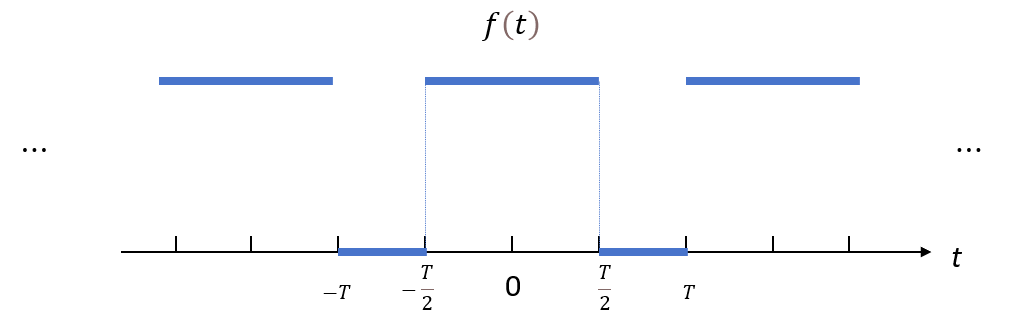
\includegraphics[scale=0.5]{1.jpg}
    \caption{时域上的一个门函数}
\end{figure}
\[  f(t) =\left\{ \begin{array}{rcl}
    1 & & {t\in (-\frac{\tau }{2} ,\frac{\tau }{2} )}\\
    0 & & {e,e}\\
    \end{array} \right. \]
\subsection{傅里叶级数展开}
$F_n=\frac{1}{T}\int_{-\frac{T }{2}}^{\frac{T}{2}}f(t)e^{-jn\Omega{t}}{\rm{dt}}$ \par
\quad \, $=\frac{1}{T}\int_{-\frac{\tau }{2}}^{\frac{\tau }{2}}e^{-jn\Omega{t}}{\rm{dt}}$\par
\quad \, $=\frac{1}{-jn\Omega{t}} e^{-jn\Omega{t}}\mid_{-\frac{\tau }{2}}^{\frac{\tau }{2}}$\par
\quad \, $=\frac{1}{jn\Omega{t}}(e^{jn\Omega{\frac{\tau }{2}}}-e^{-jn\Omega{\frac{\tau }{2}}})$,有:$cos\theta =\frac{1}{2}(e^{j\theta }+e^{-j\theta })$,$sin\theta =\frac{1}{2j}(e^{j\theta }-e^{-j\theta })$\par
\quad \, $=\frac{2}{n\Omega{t}}sin(\frac{n\Omega\tau }{2} )$\par
\quad \, $=\frac{\tau }{T}\frac{sin(\frac{n\Omega\tau }{2})}{\frac{n\Omega\tau }{2}}  $\par
令$\frac{n\Omega\tau }{2}=x$\par
\quad \, $=\frac{\tau }{T}\frac{sinx}{x}$\par
\subsection{$sinx/x$}
\begin{figure}[h]
    \centering         %使图片居中放置
    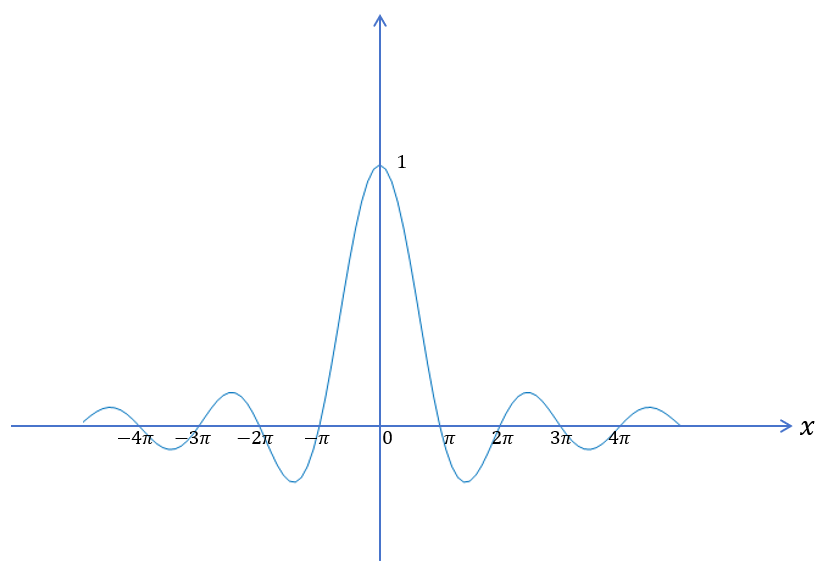
\includegraphics[scale=0.5]{2.png}
    \caption{sinc函数示意图}
\end{figure}
当将x轴弯曲为圆形时,该函数形式为雷达信号发射时的强度图 \par
\begin{figure}[h]
    \centering         %使图片居中放置
    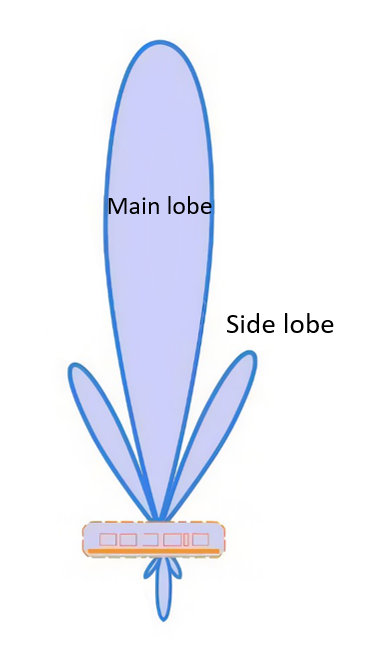
\includegraphics[scale=0.5]{3.png}
    \caption{雷达主瓣与旁瓣}
\end{figure}
(1)对于门函数傅里叶级数展开后,对应的sinc图像中每个“包络”间隔是多少?\par
$\omega =n\Omega $ \par
间隔$\omega =\frac{2\pi}{T} (rad/s) $\par
\textbf{结论1:采样间隔与$\tau $无关,只与周期T有关。}\par
(2)对于门函数傅里叶级数展开后,对应的sinc图像中$\pi$对应着多少?\par
$n\omega\tau /2 =\pi $ , $ n\Omega=\omega $  \par
于是有:\par
$\omega \frac{\tau }{2} =\pi \Longrightarrow \omega =\frac{2\pi}{\tau } $\par
\textbf{结论2:第一个“0”点(形状)及后续“0”点只由$\tau $决定,与T无关。}\par
(3)$0\thicksim \pi$之间有几条线(采样间隔)? 令$\tau=\frac{1}{4} T $\par
$\frac{2\pi }{\tau }/\frac{2\pi }{T}=\frac{T}{\tau } =4  $\par
\begin{figure}[h]
    \centering         %使图片居中放置
    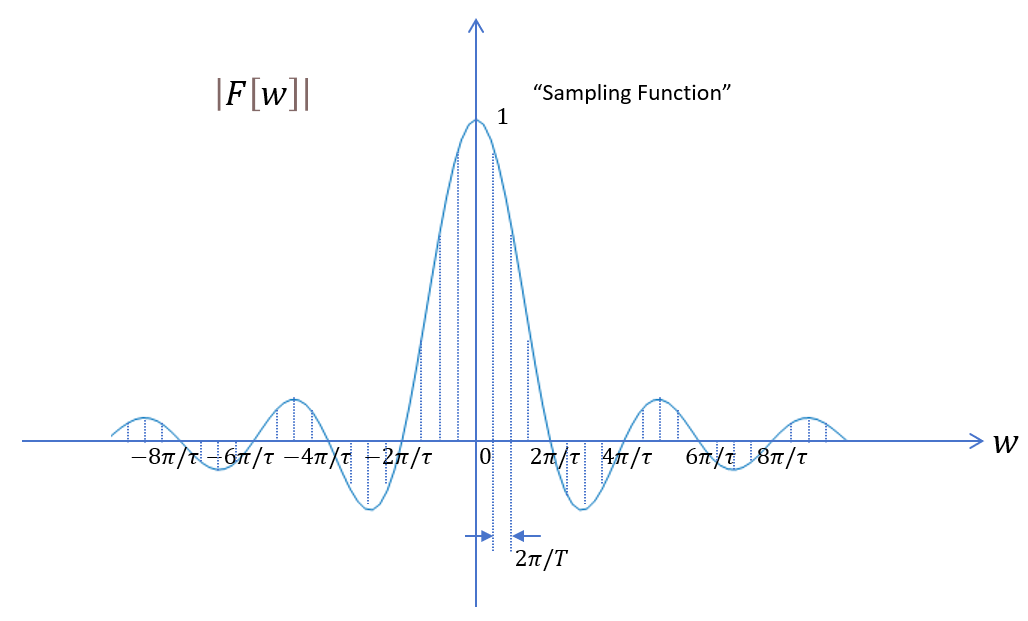
\includegraphics[scale=0.4]{4.png}
    \caption{采样函数示意图}
\end{figure}
$F_n=\frac{\tau }{T}\frac{sin(n\Omega\tau /2)}{n\Omega\tau /2}  $\par
$sinc(x)=\frac{sin(\pi x)}{\pi x} $\par
(4)当T不变,$\tau$变小,图4函数图像怎么变化?\par
\begin{figure}[h]
    \centering         %使图片居中放置
    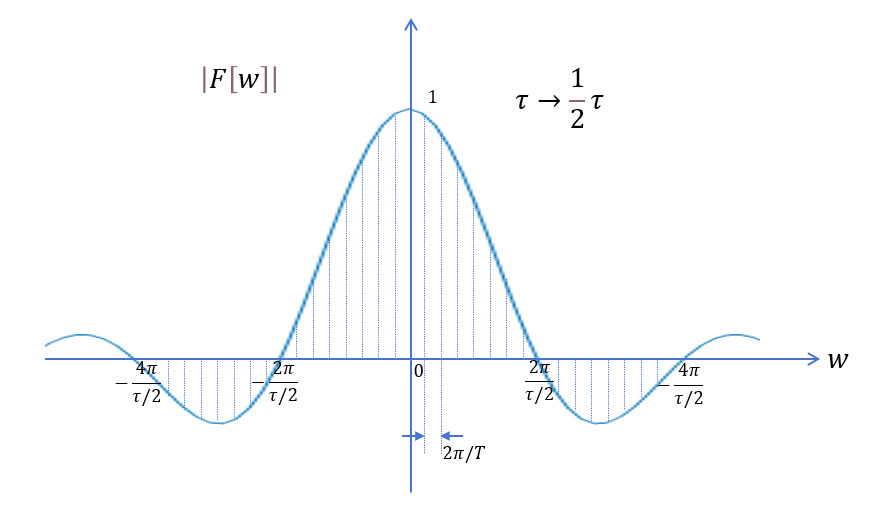
\includegraphics[scale=0.4]{5.png}
    \caption{$\tau$变小两倍}
\end{figure}
T不变$\rightarrow $采样间隔不变\par
$\tau$变小$\rightarrow\frac{2\pi}{\tau}  $变大\par

(5)当T变大,$\tau$不变,图4函数图像怎么变化?\par
T变大$\rightarrow \frac{2\pi}{T}$变小,采样间隔更密\par
$\tau$不变$\rightarrow  $第一个“0”点及之后的“0”点不变$\rightarrow $“包络”形状不变 \par
\begin{figure}[h]
    \centering         %使图片居中放置
    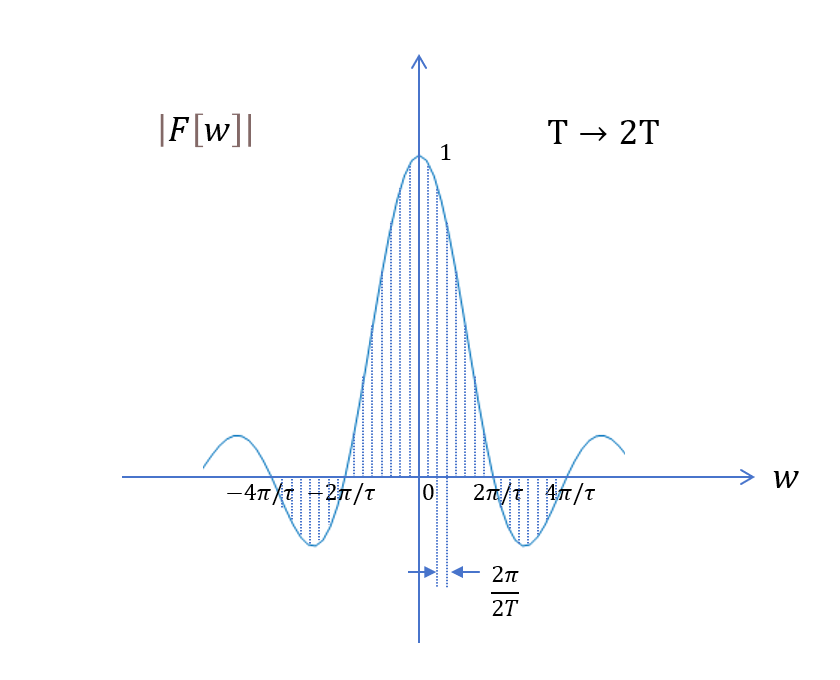
\includegraphics[scale=0.5]{6.png}
    \caption{T增大两倍}
\end{figure}

\textbf{ 结论1:周期信号T变大,采样更密,但不影响包络的形状,即不增加信息。} \par
\;\textbf{结论2:一个域“拉伸”对应着另一个域的“压缩”,反之亦然。}\par

\end{document}